% Options for packages loaded elsewhere
\PassOptionsToPackage{unicode}{hyperref}
\PassOptionsToPackage{hyphens}{url}
%
\documentclass[
]{article}
\usepackage{amsmath,amssymb}
\usepackage{lmodern}
\usepackage{iftex}
\ifPDFTeX
  \usepackage[T1]{fontenc}
  \usepackage[utf8]{inputenc}
  \usepackage{textcomp} % provide euro and other symbols
\else % if luatex or xetex
  \usepackage{unicode-math}
  \defaultfontfeatures{Scale=MatchLowercase}
  \defaultfontfeatures[\rmfamily]{Ligatures=TeX,Scale=1}
\fi
% Use upquote if available, for straight quotes in verbatim environments
\IfFileExists{upquote.sty}{\usepackage{upquote}}{}
\IfFileExists{microtype.sty}{% use microtype if available
  \usepackage[]{microtype}
  \UseMicrotypeSet[protrusion]{basicmath} % disable protrusion for tt fonts
}{}
\makeatletter
\@ifundefined{KOMAClassName}{% if non-KOMA class
  \IfFileExists{parskip.sty}{%
    \usepackage{parskip}
  }{% else
    \setlength{\parindent}{0pt}
    \setlength{\parskip}{6pt plus 2pt minus 1pt}}
}{% if KOMA class
  \KOMAoptions{parskip=half}}
\makeatother
\usepackage{xcolor}
\IfFileExists{xurl.sty}{\usepackage{xurl}}{} % add URL line breaks if available
\IfFileExists{bookmark.sty}{\usepackage{bookmark}}{\usepackage{hyperref}}
\hypersetup{
  pdftitle={Resenha artigo:},
  pdfauthor={Gabriel D'assumpção de Carvalho},
  hidelinks,
  pdfcreator={LaTeX via pandoc}}
\urlstyle{same} % disable monospaced font for URLs
\usepackage[margin=1in]{geometry}
\usepackage{longtable,booktabs,array}
\usepackage{calc} % for calculating minipage widths
% Correct order of tables after \paragraph or \subparagraph
\usepackage{etoolbox}
\makeatletter
\patchcmd\longtable{\par}{\if@noskipsec\mbox{}\fi\par}{}{}
\makeatother
% Allow footnotes in longtable head/foot
\IfFileExists{footnotehyper.sty}{\usepackage{footnotehyper}}{\usepackage{footnote}}
\makesavenoteenv{longtable}
\usepackage{graphicx}
\makeatletter
\def\maxwidth{\ifdim\Gin@nat@width>\linewidth\linewidth\else\Gin@nat@width\fi}
\def\maxheight{\ifdim\Gin@nat@height>\textheight\textheight\else\Gin@nat@height\fi}
\makeatother
% Scale images if necessary, so that they will not overflow the page
% margins by default, and it is still possible to overwrite the defaults
% using explicit options in \includegraphics[width, height, ...]{}
\setkeys{Gin}{width=\maxwidth,height=\maxheight,keepaspectratio}
% Set default figure placement to htbp
\makeatletter
\def\fps@figure{htbp}
\makeatother
\setlength{\emergencystretch}{3em} % prevent overfull lines
\providecommand{\tightlist}{%
  \setlength{\itemsep}{0pt}\setlength{\parskip}{0pt}}
\setcounter{secnumdepth}{5}
\usepackage{amsmath}
\usepackage{fancyhdr}
\usepackage{listings}
\usepackage{xcolor}
\usepackage{fvextra}
  \DefineVerbatimEnvironment{Highlighting}{Verbatim}{
    breaksymbolleft={},
    showspaces = false,
    showtabs = false,
    breaklines,
    commandchars=\\\{\}
  }
\pagestyle{fancy}
\fancyhead[L]{2º Prova}
\fancyfoot[C]{Página \thepage}
\fancyhead[C]{}

\ifLuaTeX
  \usepackage{selnolig}  % disable illegal ligatures
\fi
\usepackage[]{natbib}
\bibliographystyle{plainnat}

\title{Resenha artigo:}
\usepackage{etoolbox}
\makeatletter
\providecommand{\subtitle}[1]{% add subtitle to \maketitle
  \apptocmd{\@title}{\par {\large #1 \par}}{}{}
}
\makeatother
\subtitle{2-D Rayleigh autoregressive moving average model for SAR image modeling}
\author{Gabriel D'assumpção de Carvalho}
\date{2025-08-10}

\begin{document}
\maketitle

{
\setcounter{tocdepth}{2}
\tableofcontents
}
\hypertarget{modelo}{%
\section{Modelo}\label{modelo}}

No artigo ``2-D Rayleigh autoregressive moving average model for SAR image modeling'', os autores propõem um modelo autorregressivo e de média móvel bidimensional (2-D ARMA) para modelar imagens de radar de abertura sintética (SAR). Assume-se que as amplitudes seguem a distribuição Rayleigh, adequada por ser estritamente positiva e assimétrica, características compatíveis com sinais SAR.

O modelo é formulado como um GLM espacial com função de ligação logarítmica, resultando no 2-D RARMA(p, q). No caso RARMA(1,1), tem-se:

\[
g(\mu[n,m]) \;=\; \beta \;+\; \sum_{i=0}^{p}\sum_{j=0}^{p} \phi_{(i,j)}\, g\!\big(y[n-i,\,m-j]\big)
\;+\; \sum_{k=0}^{q}\sum_{l=0}^{q} \theta_{(k,l)}\, e[n-k,\,m-l],
\]

com \(g(\cdot)=\log(\cdot)\), em que:

\begin{itemize}
  \item \(g(\mu[n,m])\) é a média sob a ligação logarítmica;
  \item \(\beta\) é o intercepto;
  \item \(\phi_{(i,j)}\) são os parâmetros de autocorrelação espacial (parte AR);
  \item \(\theta_{(k,l)}\) são os parâmetros de média móvel espacial (parte MA);
  \item \(y[\cdot,\cdot]\) são os valores observados da imagem e \(e[\cdot,\cdot]\) os resíduos.
\end{itemize}

Como a distribuição Rayleigh tem suporte em \(\mathbb{R}^+\), a ligação log garante predições positivas, coerentes com a natureza das intensidades de radar.

Os modelos analisados incluem o 2-D RARMA(1,1), com parâmetros \(\phi_{(0,1)}, \phi_{(1,0)}, \phi_{(1,1)}\) e \(\theta_{(0,1)}, \theta_{(1,0)}, \theta_{(1,1)}\), e o 2-D RARMA(1,0), que retém apenas a componente autorregressiva, descartando a média móvel.

A estimação dos parâmetros é realizada por máxima verossimilhança condicional (CMLE), maximizando o logaritmo da densidade condicional Rayleigh em relação a cada parâmetro. O número total de parâmetros do modelo RARMA(p, q) é dado por \(( (p+1)^2 + (q+1)^2 - 1)\).

As predições são obtidas na submatriz de dimensões \(( (N - w) \times (M - w))\), onde \(( N \times M)\) representa o tamanho da imagem original e \((w = \max(p, q))\); as bordas não são estimadas devido à insuficiência de vizinhança para a recursão.

\hypertarget{teste-de-hipuxf3tese}{%
\section{Teste de hipótese}\label{teste-de-hipuxf3tese}}

Após o ajuste dos parâmetros, é possível realizar testes de hipótese com base na estatística de Wald. Os principais testes possíveis são:

\begin{enumerate}
  \item Verificar se um conjunto $\lambda_l$ de parâmetros, com dimensão $d$, é diferente do conjunto de parâmetros nulos $\lambda_{l0}$.
  \item Verificar se o conjunto total de parâmetros é diferente do conjunto nulo, ou seja, avaliar se o modelo é estatisticamente significativo.
\end{enumerate}

\hypertarget{prediuxe7uxe3o}{%
\section{Predição}\label{prediuxe7uxe3o}}

Para predizer a intensidade do pixel da imagem, utiliza-se a seguinte função:

\[
\hat{\mu}[n, m] =
\exp\!\left(
\hat{\beta} +
\sum_{i=0}^{p}\sum_{j=0}^{p} \hat{\phi}_{i,j}\, \log(y[n-i,\,m-j]) +
\sum_{k=0}^{q}\sum_{l=0}^{q} \hat{\theta}_{k,l}\, e[n-k,\,m-l]
\right)
\]

\hypertarget{detecuxe7uxe3o-de-anomalia}{%
\section{Detecção de Anomalia}\label{detecuxe7uxe3o-de-anomalia}}

Com as estimativas dos parâmetros do modelo e a estimação da intensidade do pixel, é possível detectar anomalias na imagem. Assume-se que os resíduos \(e[n, m]\) seguem uma distribuição normal com média zero e variância unitária. Assim, define-se o intervalo {[}-3, 3{]}, pois 99,7\% dos valores devem estar nesse intervalo. Estimações com resíduos fora desse intervalo são consideradas anômalas.

Além disso, foi proposto um pré-processamento da imagem para ajustar quatro modelos, cada um capturando a influência de uma direção específica: noroeste, nordeste, sudeste e sudoeste. Esse procedimento é realizado aplicando rotações de 90° na imagem.

\hypertarget{algoritmo}{%
\subsection{Algoritmo}\label{algoritmo}}

A seguir, exemplifica-se o funcionamento do algoritmo de detecção de anomalias:

\begin{enumerate}
  \item Considera-se uma imagem fictícia de 100x100 pixels;
  \item Escolhe-se uma janela de tamanho \(N \times M\);
  \item Rotaciona-se \(k\) vezes a janela em 90º;
  \item Estima-se o modelo para essa janela;
  \item Prediz-se o valor do pixel central;
  \item Calcula-se o resíduo entre a estimação e o valor observado;
  \item Verifica-se se o resíduo está dentro ou fora do intervalo \([-3, 3]\).
\end{enumerate}

Dada uma imagem de 100x100:

\begin{verbatim}
##       [,1] [,2] [,3] [,4] [,5] [,6] [,7] [,8] [,9] [,10]
##  [1,]    1    2    3    4    5    6    7    8    9    10
##  [2,]   11   12   13   14   15   16   17   18   19    20
##  [3,]   21   22   23   24   25   26   27   28   29    30
##  [4,]   31   32   33   34   35   36   37   38   39    40
##  [5,]   41   42   43   44   45   46   47   48   49    50
##  [6,]   51   52   53   54   55   56   57   58   59    60
##  [7,]   61   62   63   64   65   66   67   68   69    70
##  [8,]   71   72   73   74   75   76   77   78   79    80
##  [9,]   81   82   83   84   85   86   87   88   89    90
## [10,]   91   92   93   94   95   96   97   98   99   100
\end{verbatim}

Escolhendo uma janela de tamanho 3x3 para exemplificar o algoritmo:

\begin{verbatim}
##      [,1] [,2] [,3]
## [1,]    1    2    3
## [2,]   11   12   13
## [3,]   21   22   23
\end{verbatim}

Em seguida, realizam-se três rotações de 90º para capturar a influência das direções \emph{northwest}, \emph{northeast}, \emph{southeast} e \emph{southwest}:

\begin{verbatim}
## [1] "Northwest"
\end{verbatim}

\begin{verbatim}
##      [,1] [,2] [,3]
## [1,]    1    2    3
## [2,]   11   12   13
## [3,]   21   22   23
\end{verbatim}

\begin{verbatim}
## [1] "Northeast"
\end{verbatim}

\begin{verbatim}
##      [,1] [,2] [,3]
## [1,]    3   13   23
## [2,]    2   12   22
## [3,]    1   11   21
\end{verbatim}

\begin{verbatim}
## [1] "Southeast"
\end{verbatim}

\begin{verbatim}
##      [,1] [,2] [,3]
## [1,]   23   22   21
## [2,]   13   12   11
## [3,]    3    2    1
\end{verbatim}

\begin{verbatim}
## [1] "Southwest"
\end{verbatim}

\begin{verbatim}
##      [,1] [,2] [,3]
## [1,]   21   11    1
## [2,]   22   12    2
## [3,]   23   13    3
\end{verbatim}

Após as rotações e a estimação do modelo, cada previsão de pixel é comparada ao valor real.

\begin{itemize}
  \item Se o resíduo for maior que 3 ou menor que -3, o pixel recebe valor 0 (branco).
  \item Caso contrário, recebe valor 1 (preto).
\end{itemize}

Cada pixel terá quatro estimativas, uma para cada direção. Ao final:

\begin{itemize}
  \item Se pelo menos uma das matrizes apresentar valor 1, o pixel é considerado \textbf{normal}.
  \item Se todas apresentarem 0, o pixel é considerado \textbf{anômalo}.
\end{itemize}

Exemplo:

\begin{verbatim}
## [1] "Matriz NW"
\end{verbatim}

\begin{verbatim}
##      [,1] [,2] [,3]
## [1,]    0    0    1
## [2,]    0    1    1
## [3,]    0    1    0
\end{verbatim}

\begin{verbatim}
## [1] "Matriz NE"
\end{verbatim}

\begin{verbatim}
##      [,1] [,2] [,3]
## [1,]    1    0    0
## [2,]    0    1    1
## [3,]    1    0    1
\end{verbatim}

\begin{verbatim}
## [1] "Matriz SE"
\end{verbatim}

\begin{verbatim}
##      [,1] [,2] [,3]
## [1,]    0    0    0
## [2,]    0    0    0
## [3,]    0    0    0
\end{verbatim}

\begin{verbatim}
## [1] "Matriz SW"
\end{verbatim}

\begin{verbatim}
##      [,1] [,2] [,3]
## [1,]    0    0    0
## [2,]    0    0    0
## [3,]    0    0    0
\end{verbatim}

\begin{verbatim}
## [1] "Matriz de Detecção Final"
\end{verbatim}

\begin{verbatim}
##      [,1] [,2] [,3]
## [1,]    1    0    1
## [2,]    0    1    1
## [3,]    1    1    1
\end{verbatim}

Com isso, a detecção de anomalias, neste exemplo, identificaria que os pixels (1, 2) e (2, 1) são anômalos.

\hypertarget{resultados-dos-modelos}{%
\section{Resultados dos modelos}\label{resultados-dos-modelos}}

O artigo apresentou os resultados dos modelos 2-D RARMA(1, 0) e 2-D RARMA(1, 1), considerando dados simulados a partir do método de geração inversa da distribuição Rayleigh. Observou-se que o modelo sem médias móveis apresentou melhor desempenho para as métricas de viés relativo total e quadrado da média do erro, nos tamanhos de amostra \(10\times10\), \(20\times20\), \(40\times40\) e \(80\times80\). Para ambos os modelos, verificou-se redução dessas métricas com o aumento do tamanho da amostra.

A seleção do melhor modelo foi feita com base no teste de Wald, para verificar se os parâmetros são significativamente diferentes de zero, analisar se os resíduos se distribuem aleatoriamente em torno de zero e comparar as métricas MSE e erro percentual absoluto médio (MAPE).

\hypertarget{simulauxe7uxe3o}{%
\subsection{Simulação}\label{simulauxe7uxe3o}}

O artigo também propôs uma simulação de dados pelo método de Monte Carlo para avaliar as estimativas de cada parâmetro. A simulação consistiu nos seguintes passos:

Considerando apenas o modelo RARMA(1, 0), com parâmetros inicialmente estimados a partir de uma imagem que segue a distribuição Rayleigh: \(\beta = -0.2031\), \(\phi(0,1) = 0.4562\), \(\phi(1, 0) = 0.4523\) e \(\phi(1,1) = -0.1054\). Esses parâmetros foram tratados como valores verdadeiros. Na primeira simulação, gerou-se uma nova imagem e estimaram-se novamente os parâmetros, comparando-os com os valores verdadeiros. Esse processo foi repetido 1000 vezes, calculando-se a média final dos parâmetros, o viés relativo (\(RB = (ValorEstimado - ValorVerdadeiro) / ValorVerdadeiro\)), o erro quadrático médio e o intervalo de confiança. Em seguida, verificou-se quantas vezes os parâmetros verdadeiros estavam dentro do intervalo de confiança, obtendo o valor de CR.

\begin{center}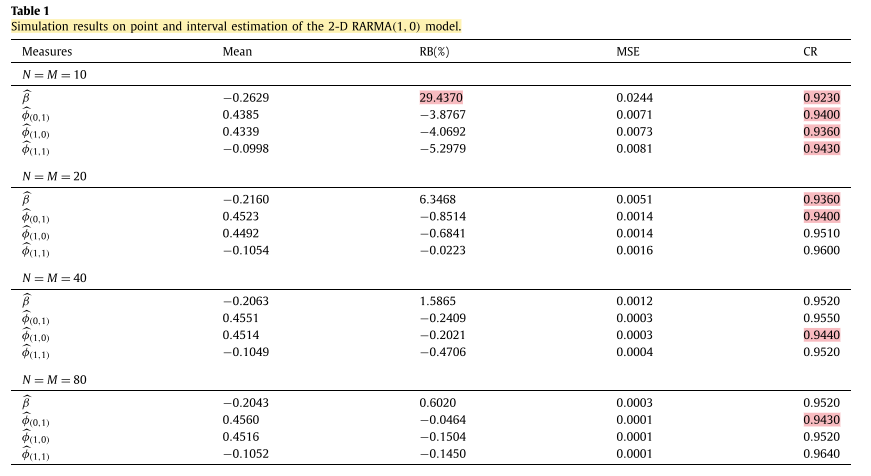
\includegraphics[width=0.6\linewidth]{table_1} \end{center}

Como podemos ver acima, quanto menor a amostra, maior é a variabilidade das estimativas dos parâmetros. Observa-se que uma amostra de \(40\times40\) já é suficientemente grande, apresentando apenas o parâmetro \(\phi(1,0)\) com maior variabilidade, estando o valor verdadeiro dentro do intervalo de confiança em 94,4\% das repetições.

\hypertarget{dados-reais}{%
\section{Dados reais}\label{dados-reais}}

Uma das aplicações do modelo foi realizada em uma imagem capturada pelo radar CARABAS II SAR, retirada de uma floresta, contendo 25 caminhões do exército, visíveis no canto superior esquerdo da imagem como 25 pontos brancos.

\begin{center}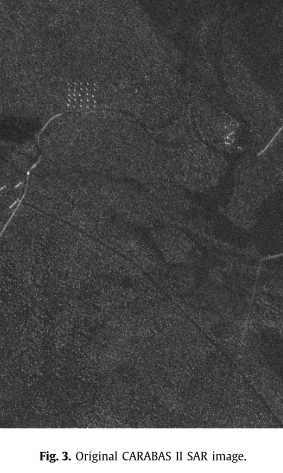
\includegraphics[width=0.3\linewidth]{carabas} \end{center}

O modelo estimado foi o seguinte:

\begin{center}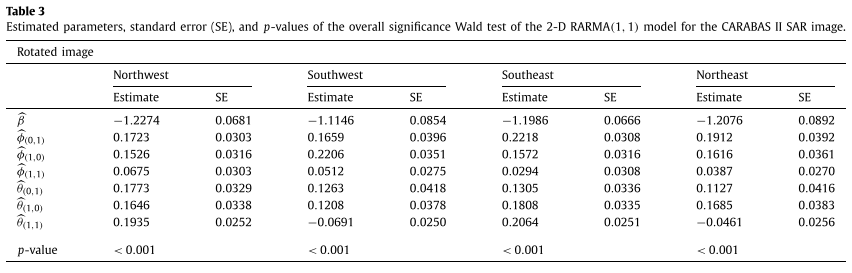
\includegraphics[width=0.7\linewidth]{table_03} \end{center}

Podemos observar na tabela acima que os quatro modelos, referentes às quatro direções, apresentaram valores-p inferiores a 0,1\% e erro padrão máximo de 0,0892. Analisando cada modelo isoladamente:

\begin{itemize}

  \item O modelo NW mostrou maior correlação no parâmetro $(\phi_{(1,1)})$, correspondente ao elemento $(n-1, m-1)$, com valor 0,1935.

  \item No modelo SW, a maior correlação foi no parâmetro $(\phi_{(1,0)})$, relativo à correlação entre o pixel $(n, m-1)$, com valor 0,2206.  

  \item Para o modelo SE, o parâmetro $(\phi_{(0,1)})$ apresentou a maior correlação, elemento $(n, m+1)$, com valor 0,2218.

  \item Por fim, o modelo NE teve maior correlação no parâmetro $(\phi_{(0,1)})$, correspondente ao pixel $(n-1, m)$, com valor 0,1906.

\end{itemize}

Os resíduos dos modelos podem ser observados na imagem abaixo, evidenciando que estão distribuídos em torno de zero e dentro do intervalo {[}-3, 3{]}, com algumas observações fora desse intervalo.

\begin{center}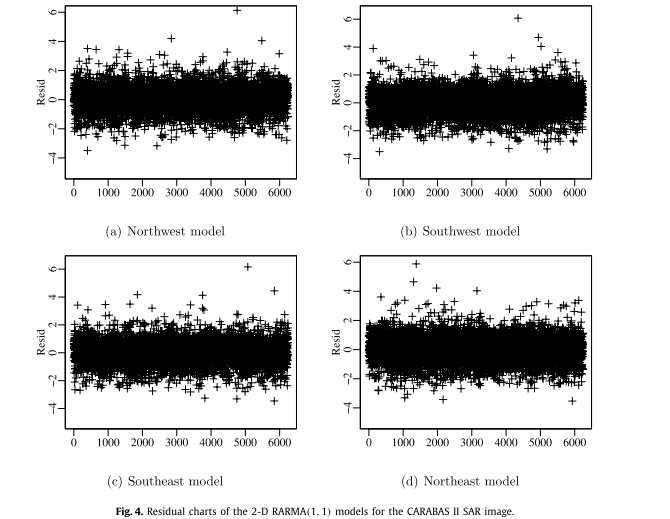
\includegraphics[width=0.7\linewidth]{fig_04} \end{center}

Em seguida, aplicou-se o algoritmo de detecção de anomalias apresentado anteriormente, resultando na imagem a seguir:

\begin{center}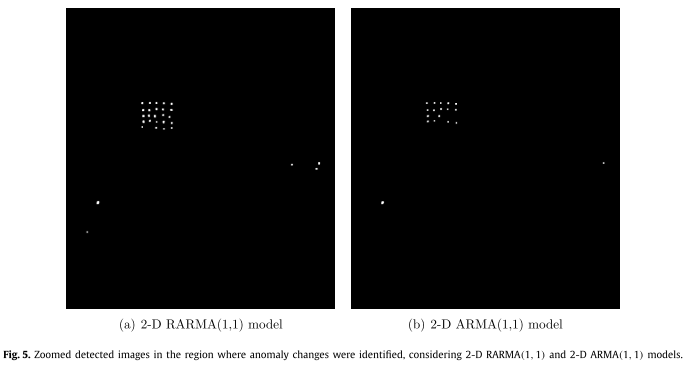
\includegraphics[width=0.7\linewidth]{fig_05} \end{center}

No lado esquerdo, observa-se que o modelo 2-D RARMA(1, 1) detectou corretamente 24 dos 25 caminhões, mas apresentou 5 erros do tipo I. Já o modelo 2-D ARMA(1, 1), que assume distribuição gaussiana, detectou 16 dos 25 caminhões e apresentou 2 erros do tipo I.

Esses resultados confirmam as vantagens do modelo 2-D RARMA para detecção de anomalias em imagens SAR conforme discutido por Palm et al.~(\citet{Palm2022}).

\renewcommand\refname{Referências}
  \bibliography{export.bib}

\end{document}
